\chapter[Introdução]{Introdução}
\label{cap:introducao}

\section{Contextualização do Tema}
A manutenção e operação eficiente de infraestruturas críticas, como subestações de energia elétrica, são fundamentais para garantir a estabilidade e a segurança do fornecimento de energia à sociedade \cite{suitelec2023}. Essas instalações, frequentemente complexas e localizadas em áreas remotas ou de difícil acesso, demandam inspeções regulares para identificar potenciais falhas, desgastes ou condições anormais que possam comprometer seu funcionamento ou representar riscos. Tradicionalmente, essas inspeções são realizadas por equipes humanas, um processo que, embora essencial, pode ser custoso, demorado, sujeito a erros humanos e, em certos casos, expor os trabalhadores a ambientes perigosos \cite{Li2025SafetyRisk}. A \autoref{fig:contextualizacao} sugere o uso de um robô quadrúpede realizando uma inspeção em uma subestação de energia elétrica.

\begin{figure}[h!]
    \centering
    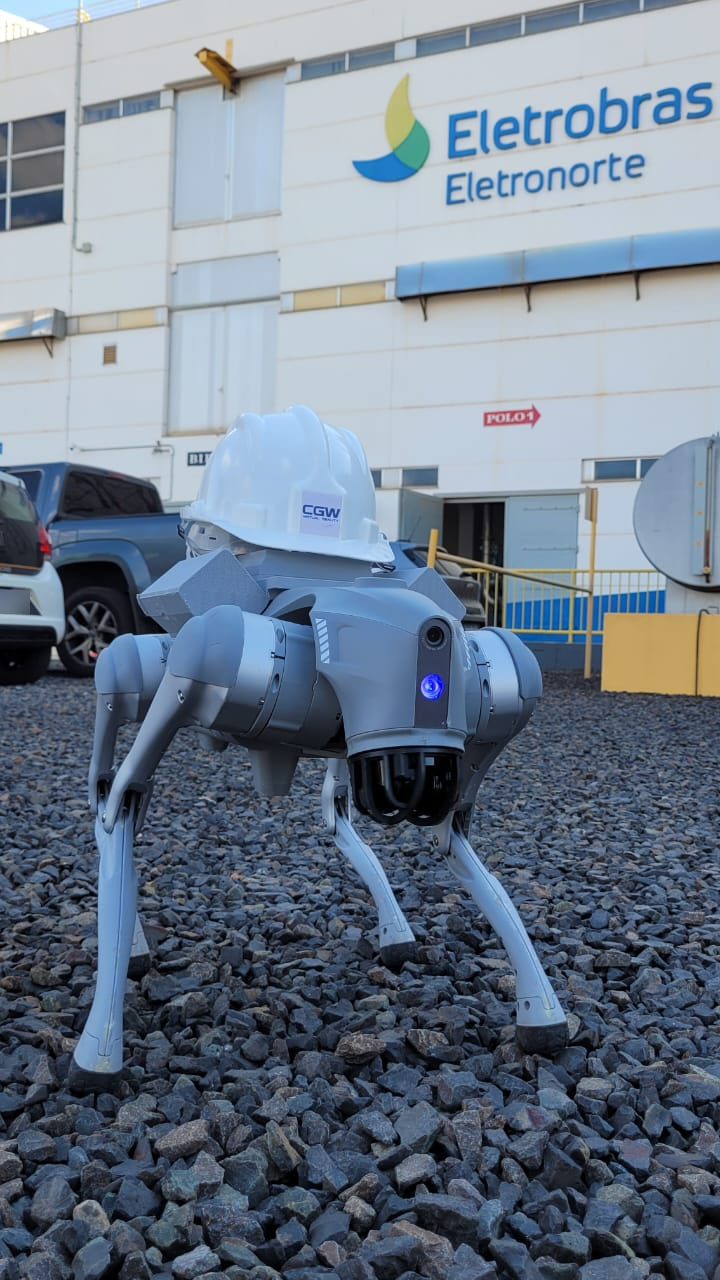
\includegraphics[width=0.8\textwidth]{figuras/fig_contextualizacao.jpg}
    \caption{Robô quadrúpede realizando inspeção em subestação de energia elétrica.}
    \legend{Fonte: O próprio autor.}
    \label{fig:contextualizacao}
\end{figure}

Nas últimas décadas, a robótica móvel autônoma emergiu como uma solução promissora para automatizar tarefas de inspeção em diversos setores industriais \cite{Wei2024Advancements}. A aplicação de robôs em subestações elétricas oferece o potencial de aumentar a frequência e a consistência das inspeções, reduzir custos operacionais, minimizar a exposição humana a riscos e coletar dados de forma mais sistemática e detalhada \cite{RobotnikSubstationBenefits}. Equipados com uma variedade de sensores, como câmeras visuais e térmicas, \ac{LiDAR}, microfones e detectores de gás, os robôs podem monitorar equipamentos, detectar anomalias como superaquecimento, descargas parciais, vazamentos ou danos estruturais e navegar autonomamente pelo ambiente complexo da subestação.
O desenvolvimento de sistemas de navegação autônoma para esses robôs é um campo de pesquisa ativo. Abordagens baseadas em \ac{SLAM} permitem que os robôs construam mapas do ambiente e se localizem dentro deles simultaneamente \cite{Kim2018SLAMMapping}. Modelos tridimensionais pré-existentes, muitas vezes gerados por técnicas como fotogrametria ou escaneamento a laser – áreas de expertise do grupo de pesquisa onde este trabalho se insere –, também podem ser utilizados para auxiliar na navegação e no planejamento de rotas. Além disso, a integração com tecnologias como \ac{RV} e \ac{RA} abre novas possibilidades para a operação remota e a visualização de dados coletados pelos robôs \cite{Ding2022QuadrupedDigitalTwin}.
Contudo, apesar dos avanços significativos, muitas das soluções atuais de inspeção robótica em subestações ainda operam predominantemente com base em rotas pré-definidas ou otimizadas para cobertura de área \cite{TJH2b2023Trends}. Essa abordagem, embora útil para tarefas de monitoramento rotineiro (ronda), pode não ser a mais eficiente ou eficaz para uma inspeção verdadeiramente investigativa. Eventos anômalos ou condições que exigem atenção imediata podem ocorrer fora da rota planejada ou exigir uma resposta dinâmica que vai além do simples seguimento de um caminho. A capacidade de um robô não apenas seguir uma rota, mas perceber ativamente seu entorno, interpretar múltiplos estímulos sensoriais de forma integrada e reagir inteligentemente a eventos inesperados, direcionando sua atenção para onde ela é mais necessária, representa um desafio e uma oportunidade significativa para a próxima geração de sistemas de inspeção autônoma.

Apesar do potencial da robótica autônoma, a implementação eficaz de sistemas de inspeção em subestações elétricas enfrenta desafios significativos que limitam o desempenho e a confiabilidade das abordagens atuais, majoritariamente baseadas em rotas pré-definidas \cite{TJH2b2023Trends}. A simples execução de rondas programadas, embora útil para cobertura sistemática, falha em abordar a necessidade de uma inspeção dinâmica e focada em eventos anômalos que podem surgir inesperadamente no ambiente complexo e muitas vezes hostil de uma subestação \cite{Wei2024Advancements}. A verdadeira inteligência em inspeção reside na capacidade do robô de perceber, interpretar e reagir adequadamente a estímulos ambientais em tempo real, adaptando sua trajetória e foco de inspeção conforme necessário.
A navegação autônoma robusta neste ambiente é particularmente desafiadora devido a uma confluência de fatores ambientais e operacionais. Primeiramente, a presença de altos níveis de interferência eletromagnética ou \ac{EMI}, inerente às operações de alta tensão, pode afetar severamente o funcionamento de sensores eletrônicos e sistemas de comunicação do robô, comprometendo a aquisição de dados e a própria capacidade de navegação \cite{He2007EMCSubstation,tdworld2024Challenges}. Sensores de localização como GPS podem ser indisponíveis ou imprecisos, a ponto de os sistemas de navegação relatados para inspeção de subestação recorrerem à combinação de DGPS com odometria \cite{Yan2024CombinedNav}, e até mesmo sensores como \ac{LiDAR} e câmeras podem sofrer interferências ou degradação de desempenho.
Adicionalmente, o ambiente físico das subestações impõe obstáculos consideráveis. A abundância de estruturas metálicas (equipamentos, grades, postes) pode causar múltiplas reflexões e oclusões para sensores baseados em ondas, como \ac{LiDAR} e radar, além de dificultar a interpretação de dados visuais \cite{Wijayathunga2023Challenges, Cai2025AttentionSeg}. A variabilidade extrema nas condições de iluminação, alternando entre luz solar direta, sombras profundas e iluminação artificial noturna, representa um desafio significativo para algoritmos de visão computacional. A necessidade de operar tanto em ambientes internos quanto externos adiciona outra camada de complexidade, exigindo que o sistema de navegação se adapte a diferentes tipos de terreno, condições atmosféricas e características espaciais \cite{Alatise2020Review}. A presença de obstáculos fixos e potencialmente dinâmicos (veículos de manutenção, pessoal) também requer capacidades avançadas de detecção e desvio.
Portanto, o problema central de pesquisa abordado nesta tese reside na \textbf{limitação dos atuais \textit{frameworks} de navegação robótica para inspeção de subestações em lidar de forma adaptativa e reativa com a complexidade ambiental e a natureza dinâmica dos eventos de interesse}. Falta uma abordagem que use a saliência do que é percebido para guiar ativamente a navegação, permitindo que o robô seja ``atraído'' por anomalias relevantes e ``repelido'' por perigos, e que o faça de modo a permitir atribuir qual mecanismo entrega qual efeito. É esse recorte --- a \emph{lógica de decisão} que arbitra entre inspecionar e se afastar, e não a cadeia de percepção que a alimenta --- que esta tese ataca. A \autoref{fig:problema_pesquisa} mostra um infográfico com uma representação do problema da pesquisa.

\section{Problema de Pesquisa}
\label{sec:intro-problema}

%% Secao preenchida em 13/11/2026. Ela existia apenas com titulo e figura, de modo
%% que a pergunta de pesquisa nao estava enunciada em lugar algum do documento. As
%% subperguntas abaixo sao, uma a uma, o contraste experimental que as responde.

Robôs de inspeção de subestações em operação seguem rondas pré-programadas: o percurso
é fixo e não se altera em função do que o robô percebe no caminho
\cite{TJH2b2023Trends,Liu2016VisualNavSubstation}. A literatura que propõe superar essa
limitação acopla percepção e reação em sistemas que percebem, decidem e se desviam ao
mesmo tempo, e relata o desempenho \emph{agregado} do conjunto. Daí decorre o problema
desta tese, que é de atribuição e não de desempenho: quando uma arquitetura desse tipo
inspeciona mais e se afasta mais de um risco do que uma ronda fixa, não se sabe
\emph{qual} de seus mecanismos produziu cada efeito --- e a comparação contra a ronda
fixa não ajuda a descobrir, porque a ronda fixa não dispõe de mecanismo algum para
deixar a rota e perde por construção.

Essa indeterminação tem consequência prática. Quem for implantar um supervisor de
inspeção precisa decidir onde investir: em perceber melhor para ponderar alvos, em
expressar o risco no planejamento deliberativo, em dar memória temporal ao sinal de
perigo, ou em nenhuma dessas coisas. Sem atribuição, a decisão é tomada por analogia
com um resultado agregado que pode ter vindo de outro componente. E há um custo que o
relato agregado esconde: uma precedência de segurança que funciona bem também recusa
inspeções legítimas, e esse preço raramente é medido.

Formula-se, assim, a pergunta central:

\begin{quote}
Em uma arquitetura de inspeção que acopla o que o robô percebe à forma como ele reage,
\emph{qual mecanismo responde por qual efeito, e a que custo} --- quando cada mecanismo
é trocado ou removido isoladamente, mantidos o mesmo controlador de navegação, o mesmo
cenário e o mesmo protocolo de medida?
\end{quote}

Ela se desdobra em seis subperguntas, cada uma amarrada a um contraste executado:

\begin{enumerate}
    \item \textbf{Origem do afastamento.} Diante de um risco \emph{estático} sobre a
    rota de patrulha, o afastamento observado é produzido pela ponderação reativa ou
    pela expressão deliberativa da repulsão no \textit{costmap}? \emph{Contraste:}
    patrulha fixa com a mesma zona de exclusão e sem supervisor reativo, contra a
    ablação que retém a inspeção reativa, contra a ablação sem zona de exclusão
    (Seção~\ref{sec:res-ablacao}).

    \item \textbf{Critério de seleção.} Ponderar o alvo por saliência produz desfecho
    diferente de simplesmente escolher o mais próximo? \emph{Contraste:} variante que
    difere \emph{apenas} na regra de seleção, nos três cenários
    (Seção~\ref{sec:res-heu}).

    \item \textbf{Modo de disparo e persistência.} Substituir o campo com limiar e
    decaimento por detecção bruta altera o desfecho de segurança quando um risco está
    colocalizado com uma anomalia mais saliente? \emph{Contraste:} heurística genérica
    de detectar--selecionar--desviar--retornar sobre o \emph{mesmo} controlador
    Nav2/MPPI (Seção~\ref{sec:res-heu}), com a ressalva de que disparo e persistência
    variam em conjunto (Seção~\ref{sec:res-ameacas}).

    \item \textbf{Custo da precedência.} Qual é o preço, em inspeções perdidas e em
    tempo de missão, de conceder prioridade categórica ao canal de risco? \emph{
    Contraste:} cenário com risco marginalmente elegível
    (Seção~\ref{sec:res-custo-precedencia}) e varreduras de limiar e de histerese
    (Seções~\ref{sec:res-sens-limiar} e~\ref{sec:res-histerese}).

    \item \textbf{Papel do aprendizado.} Uma tabela de valor treinada com recompensa
    aumentada pelo campo, \emph{selecionando} as ações, supera a regra fixa de
    precedência? \emph{Contraste:} linha de base \textsc{Q-driven} nos três cenários
    (Seção~\ref{sec:res-qdriven}).

    \item \textbf{Métrica contra propriedade física.} Quanto da completude de inspeção
    relatada é propriedade do comportamento e quanto é do critério de confirmação
    adotado? \emph{Contraste:} varredura de ruído de percepção e reavaliação
    retrospectiva do limiar de confirmação sobre os mesmos registros
    (Seções~\ref{sec:res-ruido} e~\ref{sec:res-inspecao}).
\end{enumerate}

A resposta a essas subperguntas --- inclusive quando ela é negativa, como nos itens 2
e~5 --- é o que esta tese oferece como contribuição, e não a demonstração de que um
robô de inspeção pode desviar de um obstáculo.

\begin{figure}[h]
    \centering
    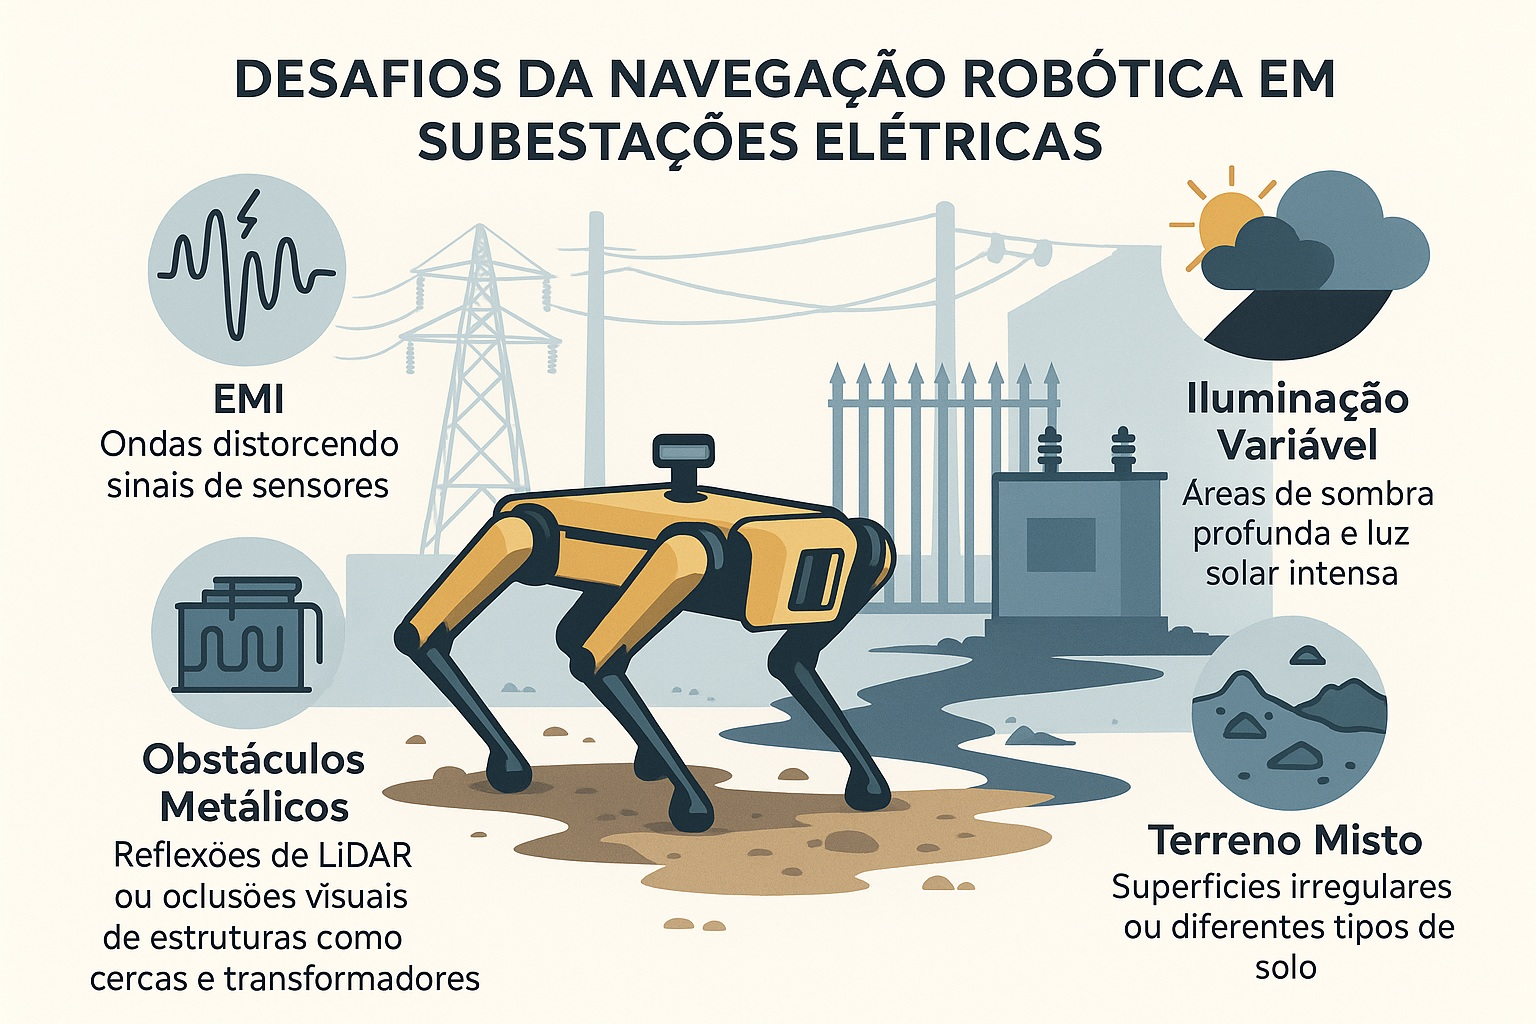
\includegraphics[width=0.8\textwidth]{figuras/fig_problema_pesquisa.jpg}
    \caption{Desafios da Navegação Robótica em Subestações Elétricas.}
    \legend{Fonte: O próprio autor.}
    \label{fig:problema_pesquisa}
\end{figure}


\section{Justificativa e Relevância}

A presente pesquisa se justifica pela necessidade premente de aprimorar os métodos de inspeção em subestações elétricas, superando as limitações das abordagens manuais e das atuais soluções robóticas baseadas em rotas. A relevância deste trabalho reside tanto em suas potenciais contribuições práticas para o setor elétrico quanto em seus avanços científicos no campo da robótica autônoma.
Do ponto de vista prático, o desenvolvimento de uma arquitetura de navegação capaz de adaptar a ronda de inspeção ao que o robô percebe tem o potencial de impactar significativamente a operação e manutenção de subestações. Ao permitir inspeções mais frequentes, consistentes e detalhadas, a solução proposta pode levar a uma detecção mais precoce de falhas e anomalias, contribuindo para a redução de custos com manutenção corretiva e minimizando o risco de interrupções no fornecimento de energia \cite{Wei2024Advancements}. A automação de tarefas de inspeção, especialmente em ambientes perigosos ou de difícil acesso, aumenta a segurança dos trabalhadores, reduzindo sua exposição a riscos elétricos e ambientais \cite{Anybotics2023Advantages}. Além disso, a capacidade de reação inteligente a eventos inesperados pode otimizar o tempo de inspeção, focando os recursos do robô nas áreas que realmente demandam atenção, aumentando a eficiência geral do processo \cite{EnergyRobotics2024Future}.
%% Reescrito em 12/11/2026. O texto anterior reivindicava fusão sensorial
%% heterogênea e aprendizado por reforço como as contribuições científicas do
%% trabalho -- promessa da proposta de qualificação que a avaliação não sustenta,
%% conforme a Seção~\ref{sec:intro-escopo}. As referências foram preservadas: elas
%% agora situam as frentes da literatura, em vez de atestar entregas desta tese.
Cientificamente, esta tese ataca uma lacuna de \emph{atribuição}. A literatura recente de navegação para inspeção avança em duas frentes --- a fusão de sensores heterogêneos, incluindo \ac{LiDAR}, visão computacional, visão térmica, áudio e ultrassom, para construir percepção situacional robusta sob oclusão e degradação sensorial \cite{Alatise2020Review, Ou2024SensorFusionDRL}, em instalação cujo rigor eletromagnético é requisito de projeto reconhecido \cite{He2007EMCSubstation}, e as políticas aprendidas para decidir como reagir ao que se percebe \cite{Zhu2017, Kahn2021} ---, e ambas relatam ganhos agregados de desempenho. O que raramente se estabelece é \emph{qual mecanismo} produz cada ganho. Um sistema que percebe, decide e desvia melhora a inspeção por várias razões simultâneas, e a comparação contra uma ronda fixa é vencida por construção, já que a ronda fixa não dispõe de mecanismo para deixar a rota. Esta tese adota a posição oposta: formula o acoplamento entre o que se percebe e como se reage como um campo escalar de atração e repulsão com precedência categórica de segurança, afastando-se tanto do planejamento de caminho puro quanto do controlador puramente reativo \cite{Wijayathunga2023Challenges}, e em seguida desmonta experimentalmente a própria proposta --- comparando-a contra uma heurística genérica executada sobre o mesmo controlador, trocando um fator de cada vez e ablacionando a resposta de segurança em seus componentes --- para declarar o que a evidência sustenta e o que não sustenta. A contribuição é esse conjunto de atribuições, inclusive as negativas, sobre uma classe de arquitetura que vem sendo adotada sem tal escrutínio. Finalmente, ao tratar dos desafios específicos das subestações elétricas, o trabalho contribui com conhecimento aplicável a outros domínios que exigem navegação robótica robusta em condições adversas.
Portanto, a pesquisa proposta é relevante por oferecer uma solução tecnológica com potencial de impacto direto na indústria de energia elétrica, ao mesmo tempo que avança o conhecimento científico em áreas chave da robótica autônoma, como a arbitragem entre comportamentos, a navegação adaptativa e a avaliação experimental de sistemas robóticos. A \autoref{fig:justificativa} ilustra a relevância da pesquisa.

\begin{figure}[h]
    \centering
    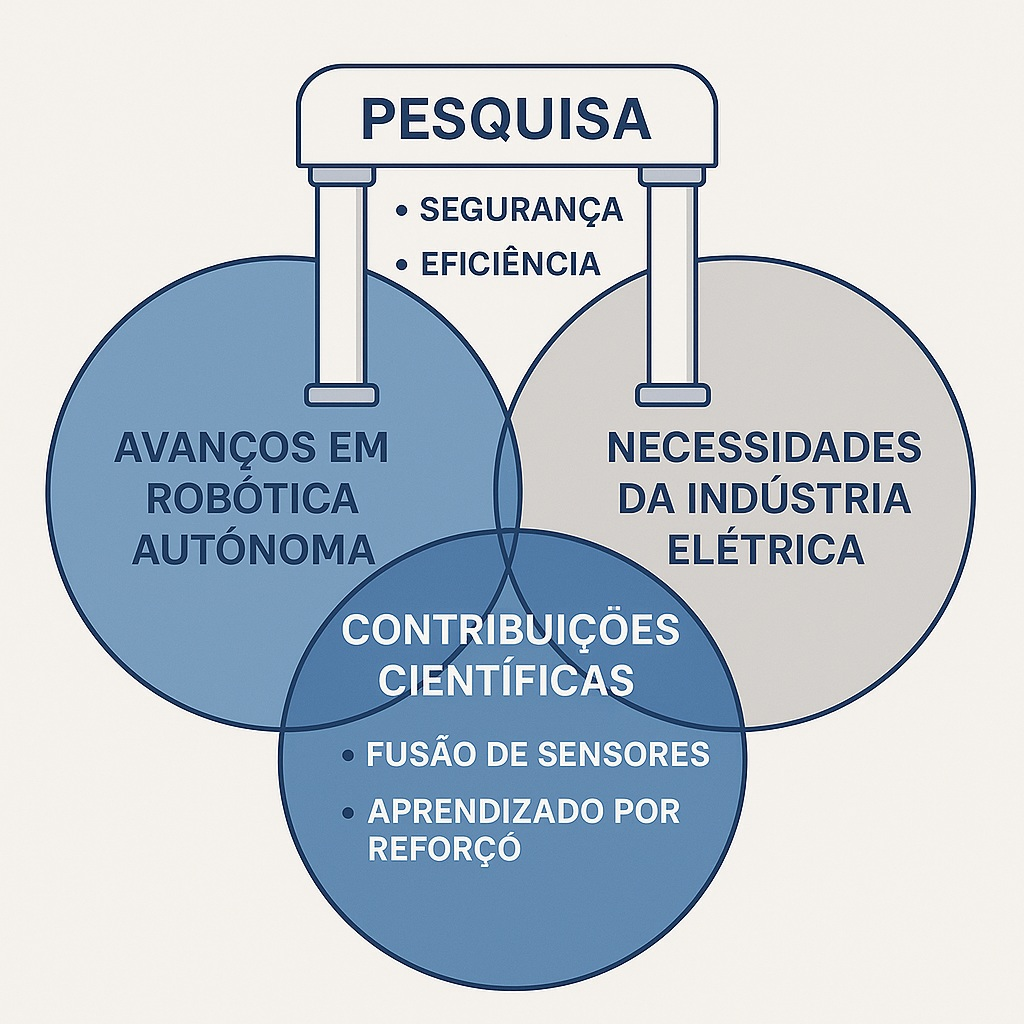
\includegraphics[width=0.8\textwidth]{figuras/fig_justificativa.jpg}
    \caption{Relevância da Pesquisa: Interseção entre Robótica Autônoma e Necessidades da Indústria Elétrica.}
    \legend{Fonte: O próprio autor.}
    \label{fig:justificativa}
\end{figure}


\section{Objetivos}

\subsection{Objetivo Geral}

Projetar, implementar e avaliar uma arquitetura de navegação deliberativo-reativa de
duas camadas para inspeção de subestações elétricas, na qual uma patrulha
deliberativa de sensoriamento ativo conduz os sensores pelo sítio e uma camada
reativa converte a saliência sensorial em um campo de atração/repulsão que aciona,
por limiar, a aproximação de anomalias e o afastamento de riscos --- atribuindo
experimentalmente a cada mecanismo o efeito que ele de fato produz.

\subsection{Objetivos Específicos}

\begin{enumerate}
    \item \textbf{Formular o campo de atração--repulsão.} Definir um campo escalar
    com memória, construído a partir de modalidade, intensidade e distância dos
    eventos percebidos, e uma regra de arbitragem que imponha segurança antes de
    inspeção como precedência categórica, e não como disputa de magnitude.

    \item \textbf{Projetar a camada reativa.} Especificar uma máquina de estados
    finitos que preempte a patrulha diante de eventos salientes, emita metas focadas
    de aproximação ou recuo a uma pilha de navegação madura e devolva o controle à
    patrulha, mantendo separadas as etapas de controle e de crédito de inspeção.

    \item \textbf{Integrar repulsão deliberativa e reativa.} Combinar o recuo
    reativo a uma zona de exclusão persistente projetada no \textit{costmap} global,
    de modo a tratar riscos que bloqueiam a própria rota de patrulha.

    \item \textbf{Avaliar com linhas de base que isolem o mecanismo.} Comparar a
    arquitetura contra uma patrulha fixa, contra um controlador de campo potencial
    artificial e --- sobretudo --- contra uma heurística genérica de
    detectar--selecionar--desviar--retornar sobre o \emph{mesmo} controlador, de
    modo a separar o campo do mero ato de desviar.

    \item \textbf{Atribuir efeitos a mecanismos por ablação.} Desmontar a resposta
    de segurança em seus componentes --- zona de exclusão, recuo reativo, ponderação
    por saliência, modo de disparo --- e medir a contribuição de cada um, declarando
    explicitamente o que a evidência sustenta e o que não sustenta.

    \item \textbf{Quantificar os custos da precedência.} Medir o preço, em inspeções
    perdidas e em tempo de missão, da prioridade rígida concedida ao canal de risco,
    em vez de tratá-lo como efeito colateral aceitável não examinado.

    \item \textbf{Entregar um pacote reprodutível.} Publicar código, mundo simulado,
    dados por execução e \textit{scripts} de análise, de modo que todo denominador
    relatado possa ser conferido.
\end{enumerate}

%% Secao criada em 13/11/2026. As contribuicoes estavam dispersas entre objetivos,
%% metodologia e conclusao, o que deixava o leitor sem saber o que e herdado, o que e
%% modificacao e qual evidencia sustenta cada uma. Cada item declara os cinco campos
%% na mesma ordem, e nenhum deles omite a limitacao.
\section{Contribuições}
\label{sec:intro-contribuicoes}

Cada contribuição é declarada em cinco campos --- componente herdado, modificação
proposta, evidência produzida, conhecimento novo e limitação ---, de modo que o que é
reivindicado como original possa ser separado do que é reaproveitado e confrontado com
a evidência correspondente. Duas das seis contribuições são \emph{resultados
negativos}: eles são declarados como contribuição porque delimitam uma classe de
arquitetura que vem sendo adotada sem esse escrutínio, e não porque confirmam a
proposta.

\begin{enumerate}
    \item \textbf{Campo de atração--repulsão com canais de memória e precedência
    categórica.} \emph{Herdado:} campos de atração e repulsão para navegação
    \cite{Arkin1989,Barraquand1992} e prioridade fixa entre camadas de comportamento
    \cite{Brooks1986}. \emph{Modificação:} o canal de risco não disputa magnitude com
    o canal de inspeção --- ele governa por precedência categórica sempre que um risco
    é elegível --- e carrega memória própria, com limiar de elegibilidade e decaimento
    (Seção~\ref{sec:prop-campo}). \emph{Evidência:} contraste contra uma heurística
    genérica de detectar--selecionar--desviar--retornar executada sobre o mesmo
    controlador Nav2/MPPI, e varreduras de limiar e de histerese
    (Seções~\ref{sec:res-heu}, \ref{sec:res-sens-limiar} e~\ref{sec:res-histerese}).
    \emph{Conhecimento novo:} nos cenários executados, o que separa esta camada de uma
    heurística de desviar e retornar é a persistência temporal do canal de risco; a
    ponderação por saliência não produziu diferença detectável no mesmo conjunto de
    condições. \emph{Limitação:} no contraste executado, o modo de disparo e a
    persistência variam em conjunto, de modo que não são fatores separáveis com as
    configurações rodadas (Seção~\ref{sec:res-ameacas}).

    \item \textbf{Expressão deliberativa da repulsão acoplada ao recuo reativo.}
    \emph{Herdado:} inflação de obstáculos em mapa de custos na pilha de navegação
    \cite{Macenski2022}. \emph{Modificação:} projeção persistente do risco detectado
    como zona de exclusão no mapa de custos global, acoplada à preempção reativa, para
    tratar riscos que bloqueiam a própria rota de patrulha
    (Seção~\ref{sec:prop-keepout}). \emph{Evidência:} ablação em três braços --- com
    zona e sem supervisor, com ambos, e sem zona (Seção~\ref{sec:res-ablacao}).
    \emph{Conhecimento novo:} sobre um risco estático na rota, o afastamento é
    atribuível à zona de exclusão deliberativa e não à ponderação reativa; e sem ela o
    recuo reativo sozinho não resolveu o risco dentro do orçamento de execução concedido
    --- nenhuma execução concluiu a missão. \emph{Limitação:} o resultado vale para o
    cenário de risco estático sobre a rota e para as configurações estudadas; ausência
    de benefício adicional detectado não demonstra equivalência geral de componentes.

    \item \textbf{Desenho de avaliação que isola o mecanismo.} \emph{Herdado:}
    protocolos de comparação por simulação em navegação autônoma. \emph{Modificação:} a
    heurística comparada roda sobre o \emph{mesmo} controlador Nav2/MPPI e a mesma
    camada de eventos, o que remove o controlador como confundidor, e cada variante
    troca um fator por vez (Capítulo~\ref{cap:avaliacao}). \emph{Evidência:} $32$ pares
    configuração--cenário, $320$ execuções tentadas e $311$ válidas, com família de
    comparação primária de $15$ testes declarada a priori quanto à regra de
    multiplicidade (Seções~\ref{sec:setup-censo} e~\ref{sec:res-familias}).
    \emph{Conhecimento novo:} o ganho sobre uma ronda fixa não é informativo sobre
    mecanismo; o contraste informativo é contra a mesma arquitetura com um fator
    trocado. \emph{Limitação:} um único \textit{layout} e uma única distribuição de
    eventos por cenário --- o que as repetições estabelecem é repetibilidade naquelas
    condições, não validade externa.

    \item \textbf{Custo medido da precedência de segurança.} \emph{Herdado:} a prática
    de dar prioridade à segurança, corrente desde as arquiteturas em camadas.
    \emph{Modificação:} um cenário desenhado para tornar esse custo \emph{observável},
    com um risco marginalmente elegível cuja presença não justifica o recuo
    (Seção~\ref{sec:res-custo-precedencia}). \emph{Evidência:} supressão da atração por
    cerca de $70$~s e renúncia a uma de quatro inspeções em $10/10$ execuções.
    \emph{Conhecimento novo:} a precedência categórica tem preço quantificável e
    reprodutível, em inspeções perdidas e em tempo de missão, em vez de efeito
    colateral aceitável não examinado. \emph{Limitação:} o valor depende do limiar de
    elegibilidade e da geometria do cenário, e não é uma constante da arquitetura.

    \item \textbf{Resultado negativo: o critério de seleção não teve efeito
    detectável.} \emph{Herdado:} a ponderação de alvos por saliência.
    \emph{Modificação:} variante que difere \emph{apenas} na regra de seleção ---
    o alvo mais próximo em lugar do mais saliente (Seção~\ref{sec:res-heu}).
    \emph{Evidência:} desfechos discretos idênticos ao longo das dez execuções nos
    cenários de referência e distribuições sobrepostas no cenário adverso, com
    equivalência declarada por \ac{TOST} onde as margens a sustentam
    (Seção~\ref{sec:res-equivalencia}). \emph{Conhecimento novo:} nestes cenários, a
    saliência não domina a proximidade, o que redireciona o esforço de projeto para a
    arbitragem e sua extensão temporal. \emph{Limitação:} não detectar diferença não é
    equivalência, exceto onde o \ac{TOST} a declara com margem justificada; e a
    utilidade da saliência em outras distribuições de eventos não é eliminada.

    \item \textbf{Resultado negativo: a tabela de valor não substitui a regra de
    precedência.} \emph{Herdado:} \textit{Q-learning} tabular com recompensa aumentada.
    \emph{Modificação:} além da atualização passiva do método principal
    (Seção~\ref{sec:prop-atualizacao}), uma linha de base em que a tabela de valor
    \emph{seleciona} a ação executada, medida nos três cenários
    (Seção~\ref{sec:res-qdriven}). \emph{Evidência:} bloco de doze testes com correção
    interna de multiplicidade. \emph{Conhecimento novo:} a tabela de valor treinada com
    recompensa aumentada pelo campo não superou a regra fixa de precedência nas
    implementações comparadas. \emph{Limitação:} a comparação é entre as duas
    implementações efetivamente testadas --- a política atua em velocidade e foi
    treinada em simulador cinemático, enquanto o método envia metas ao Nav2/MPPI ---, e
    não entre os paradigmas de decisão em geral.
\end{enumerate}

Um sétimo item é artefato, e não conhecimento: o pacote reprodutível
--- código, mundo simulado, manifesto por execução e \textit{scripts} que regeneram as
tabelas de resultado a partir dos registros ---, cuja limitação está declarada no
Capítulo~\ref{cap:resultados}: as baterias já executadas não gravaram o identificador
de \textit{commit} por execução, o que não é recuperável retroativamente.

%% Secao criada em 12/11/2026. Registra, de frente e na introducao, o estreitamento
%% de escopo em relacao a proposta qualificada em 12/09/2026. O enquadramento e
%% deliberado: a decisao e do autor e a justificativa e a evidencia das proprias
%% simulacoes. A Secao~\ref{sec:conc-escopo} faz a retrospectiva e remete a esta.
\section{Delimitação de Escopo}
\label{sec:intro-escopo}

A proposta qualificada previa um \textit{framework} de cinco módulos --- aquisição
multissensorial, fusão sensorial heterogênea, detecção de eventos, decisão por
aprendizado por reforço e controle reativo integrado a \ac{SLAM} e a modelos
tridimensionais ---, no qual a decisão de aproximar-se de uma anomalia ou afastar-se
de um risco seria \emph{aprendida}. O que esta tese entrega é mais estreito e mais
fundo: a arquitetura de duas camadas do Capítulo~\ref{cap:proposta}, submetida a um
desenho experimental que atribui a cada mecanismo o efeito que ele de fato produz. O
estreitamento foi decidido ao longo do desenvolvimento, e decidido pelos resultados.
Cabe dizer quais resultados, e com que consequências.

\begin{enumerate}
    \item \textbf{O ganho de segurança não vem da ponderação reativa.} Uma patrulha
    fixa portando a mesma zona de exclusão disparada por detecção, e sem qualquer
    supervisor reativo, alcançou afastamento mínimo mediano de $1{,}73$~m, contra
    $1{,}71$~m da ablação que retém a inspeção reativa --- sem diferença
    estatisticamente detectável ($p_{\mathrm{Holm}}=0{,}4194$). O que a camada
    reativa acrescenta sobre a patrulha fixa são as inspeções ($3$ contra $0$ de
    $3$), não o afastamento. Um \textit{framework} organizado em torno da modulação
    do sinal de resposta estaria, portanto, organizado em torno do componente errado.

    \item \textbf{A tabela de valor não seleciona as ações executadas.} As transições
    da máquina de estados leem o campo bruto $\Phi$, e não o peso afetivo $\eta$ da
    atualização de valor; o movimento provém das metas enviadas ao Nav2/MPPI. Em
    consequência, uma varredura sobre $\eta$ não mede sensibilidade comportamental,
    e nenhum experimento conduzido atribuiu efeito observável à atualização. Treinar
    uma política sobre essa tabela exigiria política de exploração, mapeamento de
    ação para velocidade e comparação contra \textit{Q-learning} tabular comum ---
    um estudo próprio, e não um módulo a mais. Esse estudo foi posteriormente
    conduzido em sua forma executada e é relatado na Seção~\ref{sec:res-qdriven}:
    uma política tabular aprendida, selecionando a ação executada, não altera a
    completude de inspeção nem a segurança, e custa tempo na subtarefa reativa.

    \item \textbf{Percepção e localização realistas impediriam a atribuição.} Com uma
    cadeia de percepção real e localização estimada em tempo de execução, o erro de
    detecção e o erro de localização dominam a variância dos desfechos medidos.
    Diferenças de meio metro em afastamento mínimo, ou de dezenas de segundos em
    atraso de inspeção, deixam de ser atribuíveis à regra de arbitragem --- que é
    precisamente o objeto desta tese.
\end{enumerate}

Diante disso, três decisões de projeto foram tomadas, e são declaradas aqui como
\emph{controles de confundimento}, não como omissões. A saída da cadeia de percepção
foi abstraída em eventos --- modalidade, intensidade e posição ---, conforme a
Seção~\ref{sec:prop-sensoriamento}. A transformada de localização foi mantida fixa.
E a atualização de valor foi registrada como nota de projeto na
Seção~\ref{sec:prop-atualizacao}, com a ressalva explícita de que não governa o
comportamento avaliado. O preço dessas três escolhas é a validade externa: os
resultados falam da lógica de decisão da arquitetura, e não de um sistema pronto para
implantação, como a Seção~\ref{sec:prop-nao-abordado} delimita. O que elas compram é
a validade interna que torna a atribuição possível.

O objeto da tese, portanto, deslocou-se de \emph{integrar} para \emph{atribuir}. Essa
troca não reduziu a exigência experimental; aumentou-a. Onde a proposta previa
comparação contra métodos de rotas pré-definidas, a avaliação do
Capítulo~\ref{cap:avaliacao} acrescenta um controlador de campo potencial artificial,
uma heurística genérica de detectar--selecionar--desviar--retornar executada sobre o
\emph{mesmo} controlador Nav2/MPPI, variantes de um único fator e ablações da
resposta de segurança, com tamanhos de efeito, intervalos de confiança, testes
livres de distribuição e de equivalência, correção de Holm e denominadores
explícitos.

Nada do que a proposta reuniu foi descartado do documento. A fundamentação sobre
fusão sensorial heterogênea e aprendizado por reforço permanece nos
Capítulos~\ref{cap:fundamentacao} e~\ref{cap:revisao}, porque é o contexto que
motivou a investigação e que situa a arquitetura entre as alternativas. A
heterogeneidade sensorial permanece no modelo de eventos, que distingue as
modalidades térmica, acústica e de risco com parâmetros próprios. A formulação de
valor permanece como nota de projeto, com o resíduo completo reportado no
Capítulo~\ref{cap:resultados}. O que mudou foi o que se \emph{reivindica} como
entregue e demonstrado. A Tabela~\ref{tab:intro-escopo} faz essa correspondência,
objetivo por objetivo.

\begin{table}[htb]
\centering
\caption{Correspondência entre os objetivos específicos da proposta de qualificação e
o que esta tese entrega.}
\label{tab:intro-escopo}
\footnotesize
\begin{tabular}{p{0.30\textwidth}p{0.17\textwidth}p{0.42\textwidth}}
\hline
\textbf{Objetivo da proposta} & \textbf{Situação} & \textbf{Onde está nesta tese}\\
\hline
Propor arquitetura modular (fusão, detecção, decisão aprendida, controle integrado a
\ac{SLAM} e modelos 3D) &
Entregue em forma modificada &
Arquitetura de duas camadas do Capítulo~\ref{cap:proposta}, com abstração de eventos
no lugar do módulo de fusão e acionamento por limiar no lugar da decisão aprendida\\
\hline
Investigar e implementar técnicas de fusão sensorial &
Não entregue &
Tratada como fundamentação (Capítulos~\ref{cap:fundamentacao}
e~\ref{cap:revisao}); substituída pela abstração de eventos
(Seção~\ref{sec:prop-sensoriamento}) e nomeada em trabalhos futuros
(Seção~\ref{sec:conc-futuro})\\
\hline
Desenvolver e treinar modelo de aprendizado por reforço &
Entregue como formulação, análise e comparação executada &
Seção~\ref{sec:prop-atualizacao}; resíduo completo
$|\alpha\delta+\eta\Phi|$ no Capítulo~\ref{cap:resultados}; e baseline
\textsc{Q-driven} --- tabela $Q$ treinada com recompensa aumentada por $\Phi$,
selecionando a ação executada --- medido contra o método nos três cenários
(Seção~\ref{sec:res-qdriven})\\
\hline
Integrar com \ac{SLAM} e modelos tridimensionais &
Não entregue como proposto &
Transformada de localização mantida fixa, por controle de confundimento
(Seção~\ref{sec:prop-nao-abordado})\\
\hline
Validar por simulação contra métodos de rotas pré-definidas &
Entregue e ampliado &
Capítulo~\ref{cap:avaliacao}: além da patrulha fixa, campo potencial artificial,
heurística genérica sobre o mesmo controlador, variantes de um fator e ablações,
com tratamento estatístico completo\\
\hline
\end{tabular}
\end{table}

\section{Metodologia}

A abordagem adotada foi construtiva e experimental. A pesquisa foi conduzida nas
seguintes fases:

\begin{enumerate}
    \item \textbf{Revisão da literatura.} Revisão crítica da
    literatura em robótica móvel autônoma, navegação em ambientes complexos, fusão
    de sensores heterogêneos, aprendizado por reforço aplicado à robótica e inspeção
    de subestações elétricas, consolidando o estado da arte e identificando as
    lacunas que o trabalho ataca (Capítulos~\ref{cap:fundamentacao}
    e~\ref{cap:revisao}).

    \item \textbf{Projeto da arquitetura.} Definição da separação em camada
    deliberativa e camada reativa, da formulação do campo com seus dois canais de
    memória, da regra de precedência e da máquina de estados, bem como da expressão
    deliberativa da repulsão (Capítulo~\ref{cap:proposta}).

    \item \textbf{Implementação.} Implementação como pacotes ROS~2 Humble, com
    navegação pela pilha Nav2 (planejador global NavfnPlanner e controlador MPPI) e
    simulação física em Gazebo Fortress. A saída da cadeia de percepção foi
    abstraída como eventos --- modalidade, intensidade e posição ---, simplificação
    deliberada e delimitada, discutida na Seção~\ref{sec:prop-nao-abordado}.

%% Corrigido em 13/11/2026: a contagem anterior ("vinte configuracoes") nao fechava
    %% com a matriz nem com os dados em disco. O censo da Tabela~\ref{tab:setup-censo} da
    %% 32 pares configuracao-cenario e 320 execucoes tentadas.
    \item \textbf{Avaliação experimental.} Execução de uma matriz de $32$ pares
    configuração--cenário sobre seis cenários, com dez execuções tentadas por par ---
    $320$ ao todo, das quais $311$ válidas ---, abrangendo linhas de base, ablações,
    cenários de conflito e de risco emergente, varreduras de limiar e de histerese e
    perturbações de ruído de percepção (Capítulo~\ref{cap:avaliacao}, com o censo na
    Seção~\ref{sec:setup-censo}).

    \item \textbf{Análise estatística.} Comparações por testes livres de
    distribuição, com tamanhos de efeito, intervalos \textit{bootstrap} e correção
    de multiplicidade dentro de uma família de comparação declarada, mantendo
    explícita a fronteira entre alegações primárias e exploratórias
    (Capítulo~\ref{cap:resultados}).
\end{enumerate}

A \autoref{fig:metodologia} apresenta um fluxograma da metodologia geral.

\begin{figure}[h]
    \centering
%% Figura refeita em 12/11/2026. A versao anterior (fig_metodologia.jpg, ainda em
%% figuras/ mas nao mais referenciada) trazia "PROJETO E DESENVOLVIMENTO DO
%% FRAMEWORK" e "IMPLEMENTACAO E TREINAMENTO DOS COMPONENTES CHAVE" -- vocabulario
%% da proposta de qualificacao. Nao houve treinamento, e as fases agora sao as
%% efetivamente executadas, na mesma ordem do texto desta secao.
    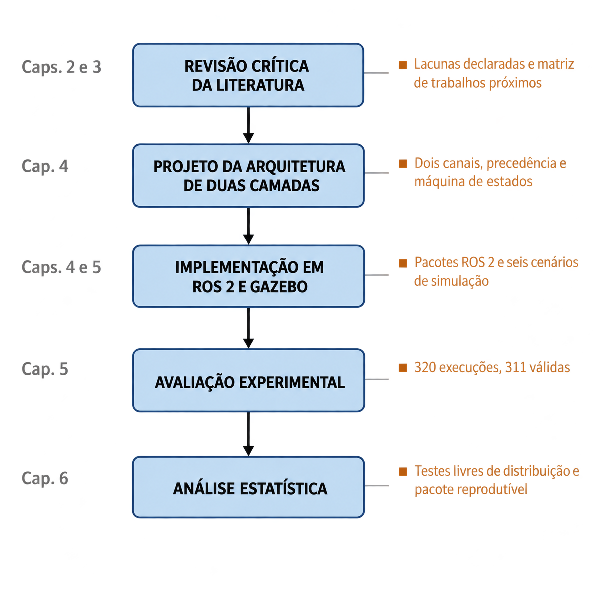
\includegraphics[width=0.8\textwidth]{figuras/fig_metodologia.pdf}
    \caption{Fluxograma da metodologia adotada.}
    \legend{Fonte: O próprio autor.}
    \label{fig:metodologia}
\end{figure}

\section{Organização do Documento}

\begin{itemize}
    \item \textbf{Capítulo~\ref{cap:introducao} --- Introdução.} Contextualiza a
    inspeção robótica em subestações, define o problema de pesquisa, justifica a
    relevância do trabalho, estabelece os objetivos, delimita o escopo em relação à
    proposta de qualificação (Seção~\ref{sec:intro-escopo}) e descreve a metodologia
    adotada.

    \item \textbf{Capítulo~\ref{cap:fundamentacao} --- Fundamentação Teórica.}
    Apresenta os fundamentos de fusão sensorial heterogênea, aprendizado por reforço,
    características operacionais de subestações elétricas, sistemas robóticos e
    ROS/ROS2, e navegação reativa em robótica móvel.

%% Renomeado em 13/11/2026 junto com o Capitulo~\ref{cap:revisao}: nao ha protocolo
    %% de revisao sistematica executado, e o capitulo agora declara seu criterio de
    %% selecao e o alcance dele.
    \item \textbf{Capítulo~\ref{cap:revisao} --- Revisão Crítica da Literatura.}
    Discute o estado da arte nas áreas relevantes, declara como os trabalhos foram
    selecionados e identifica as lacunas que esta pesquisa visa preencher.

    \item \textbf{Capítulo~\ref{cap:proposta} --- Arquitetura Proposta.} Detalha a
    arquitetura de duas camadas: o campo de atração--repulsão e seus canais com
    memória, a regra de precedência categórica, a máquina de estados
    \textsc{Stay Alert}, a zona de exclusão deliberativa e a abstração de eventos.

    \item \textbf{Capítulo~\ref{cap:avaliacao} --- Avaliação Experimental.} Descreve
    o ambiente de simulação, os cenários, a matriz experimental, as métricas, os
    hiperparâmetros e o pacote de reprodutibilidade.

    \item \textbf{Capítulo~\ref{cap:resultados} --- Resultados e Discussão.}
    Apresenta os resultados, atribui efeitos a mecanismos por ablação, quantifica os
    custos da precedência de segurança e enumera as ameaças à validade.

    \item \textbf{Capítulo~\ref{cap:conclusao} --- Conclusão.} Sintetiza as
    atribuições estabelecidas, delimita os limites da evidência, retoma a delimitação de escopo da
    Seção~\ref{sec:intro-escopo} e aponta direções para trabalhos futuros.
\end{itemize}
